% =============================================================================
% KitPri v4 — Engineering Report
% Samsung PRISM Worklet 25ST31BMS · B.M.S. College of Engineering
%
% Fully self-contained: no external figures — all diagrams are TikZ and all
% plots are pgfplots with data inlined from results/*/training_log.csv,
% student_threshold_sweep.csv, run_summary.json and quantization_report.json.
%
% Compile: pdflatex (twice) · latexmk -pdf · tectonic · or upload to Overleaf.
% =============================================================================
\documentclass[11pt,a4paper]{article}

\usepackage[margin=2.4cm]{geometry}
\usepackage{amsmath,amssymb}
\usepackage{booktabs}
\usepackage{multirow}
\usepackage{graphicx}
\usepackage{xcolor}
\usepackage{tikz}
\usetikzlibrary{arrows.meta,positioning,shapes.geometric,fit}
\usepackage{pgfplots}
\pgfplotsset{compat=1.17}
\usepackage{caption}
\captionsetup{font=small,labelfont=bf}
\usepackage{enumitem}
\usepackage{microtype}
\usepackage[hidelinks,colorlinks=true,linkcolor=blue!55!black,citecolor=blue!55!black,urlcolor=blue!55!black]{hyperref}

\definecolor{kpblue}{RGB}{28,80,150}
\definecolor{kporange}{RGB}{214,116,20}
\definecolor{kpgreen}{RGB}{34,120,66}
\definecolor{kpgray}{RGB}{110,110,110}

\newcommand{\cooking}{\textsc{Cooking}}
\newcommand{\notcooking}{\textsc{Not-Cooking}}

\title{\textbf{KitPri v4: Cooking-Sound Detection for SmartThings Edge Devices
via Cross-Architecture Knowledge Distillation and INT8 Quantization}\\[0.6em]
\large Samsung PRISM --- Worklet 25ST31BMS}
\author{Ayush Pandey\\
B.M.S.\ College of Engineering, Bengaluru\\
\texttt{github.com/ayushpandey0201/kitpribot}}
\date{July 2026}

\begin{document}
\maketitle

% -----------------------------------------------------------------------------
\begin{abstract}
\noindent
We present KitPri~v4, a complete, reproducible pipeline that detects cooking
activity from 10-second audio clips and fits the resource envelope of a
Samsung SmartThings edge device ($\sim$60\,MB RAM budget, CPU-only inference).
A 329\,MiB Audio Spectrogram Transformer (AST) teacher (86.2\,M parameters,
test F1 $0.8129$) is distilled into a 2.23\,M-parameter MobileNetV2 student
(8.49\,MB, test F1 $0.7318$ after validation-only threshold tuning), which is
then compressed by static post-training INT8 quantization to a
\textbf{2.80\,MB} TorchScript artifact (test F1 $0.6910$) --- an end-to-end
compression of more than $118\times$ with a $2.25\times$ CPU speed-up
(57.3\,$\rightarrow$\,25.5\,ms per clip). Training data is a purpose-built
corpus of 7{,}200 synthetic mixtures of 2--4 layered sound sources, including
an adversarially hard overlap regime in which the cooking source can be up to
5\,dB \emph{quieter} than a competing sound. The evaluated model is served
end-to-end through a single shared \texttt{Predictor} code path --- CLI, batch
evaluation, and a public Telegram bot hosted 24/7 on an Oracle Cloud
Always-Free VM under systemd supervision at zero recurring cost. We report
methodology, results, deployment architecture, failure modes, and open
limitations in full.
\end{abstract}

% -----------------------------------------------------------------------------
\section{Introduction}\label{sec:intro}

Ambient acoustic sensing is a natural fit for smart-home platforms: cooking
produces a rich, sustained acoustic signature (sizzling, boiling, chopping,
exhaust hum) that a microphone-equipped hub can observe passively. A reliable
\cooking{}/\notcooking{} signal enables downstream SmartThings automations ---
ventilation control, safety timers, presence inference --- without cameras or
wearables.

The engineering obstacle is not accuracy in isolation; it is accuracy
\emph{under an edge budget}. State-of-the-art audio classifiers are
transformers with hundreds of megabytes of weights, while the deployment
target offers roughly 60\,MB of RAM, no accelerator, and a CPU that must share
time with the rest of the hub's workload. KitPri~v4 addresses this gap with a
three-stage compression pipeline (Figure~\ref{fig:pipeline}) and treats
everything around the model --- dataset realism, preprocessing parity,
threshold governance, packaging, and hosting --- as first-class engineering
concerns.

\paragraph{Contributions.}
\begin{enumerate}[itemsep=2pt,topsep=3pt]
  \item A synthetic-mixture dataset methodology (7{,}200 clips) in which
        \emph{every} clip layers 2--4 sources at varying relative gains,
        deliberately including a hard overlap regime (Section~\ref{sec:data}).
  \item A benchmarked architecture selection: six EfficientNet-B0 variants
        plateau on v4 data while AST exceeds them within one epoch
        (Section~\ref{sec:teacher}).
  \item A cross-architecture distillation recipe (transformer
        $\rightarrow$ CNN) with an explicit, documented loss convention
        (Section~\ref{sec:distill}).
  \item A quantization study demonstrating why dynamic PTQ fails for
        CNN-style models and static PTQ succeeds, with measured
        size/latency/accuracy trade-offs (Section~\ref{sec:quant}).
  \item A deployment architecture with strict train/serve parity through one
        shared \texttt{Predictor}, an x86-only-artifact guard, Docker
        packaging, and a zero-cost, always-on cloud demonstration bot
        (Section~\ref{sec:deploy}).
  \item An honest limitations register, including error concentration on
        overlapped audio and an un-retuned INT8 threshold
        (Section~\ref{sec:limits}).
\end{enumerate}

% -----------------------------------------------------------------------------
\begin{figure}[t]
\centering
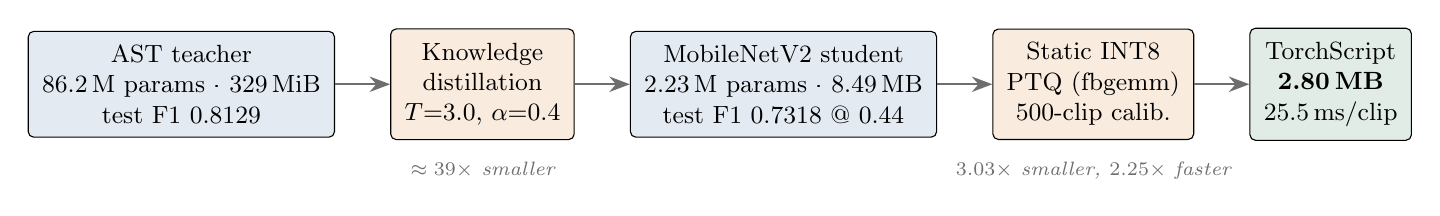
\begin{tikzpicture}[
  node distance=5.5mm and 7mm,
  stage/.style={draw, rounded corners=2pt, align=center, font=\small,
                minimum height=9mm, inner sep=5pt},
  arr/.style={-{Stealth[length=2.6mm]}, thick, kpgray},
  lab/.style={font=\scriptsize\itshape, text=kpgray}
]
\node[stage, fill=kpblue!12]   (ast)  {AST teacher\\ 86.2\,M params · 329\,MiB\\ test F1 0.8129};
\node[stage, fill=kporange!14, right=of ast] (kd)   {Knowledge\\ distillation\\ $T{=}3.0$, $\alpha{=}0.4$};
\node[stage, fill=kpblue!12,   right=of kd]  (mnv2) {MobileNetV2 student\\ 2.23\,M params · 8.49\,MB\\ test F1 0.7318 @ 0.44};
\node[stage, fill=kporange!14, right=of mnv2](ptq)  {Static INT8\\ PTQ (fbgemm)\\ 500-clip calib.};
\node[stage, fill=kpgreen!14,  right=of ptq] (ts)   {TorchScript\\ \textbf{2.80\,MB}\\ 25.5\,ms/clip};
\draw[arr] (ast) -- (kd);
\draw[arr] (kd) -- (mnv2);
\draw[arr] (mnv2) -- (ptq);
\draw[arr] (ptq) -- (ts);
\node[lab, below=1.5mm of kd]  {$\approx 39\times$ smaller};
\node[lab, below=1.5mm of ptq] {$3.03\times$ smaller, $2.25\times$ faster};
\end{tikzpicture}
\caption{The KitPri v4 compression pipeline: $>118\times$ end-to-end size
reduction from teacher checkpoint to deployed artifact.\protect\footnotemark}
\label{fig:pipeline}
\end{figure}
\footnotetext{Computed conservatively as $329/2.80$. Converting the teacher
checkpoint strictly to MB ($329\,\text{MiB} \approx 345\,\text{MB}$) yields
$123\times$.}

% -----------------------------------------------------------------------------
\section{Background and Related Work}\label{sec:related}

\textbf{Audio Spectrogram Transformer (AST)}~\cite{gong2021ast} applies a
ViT-style patch attention mechanism directly to log-mel spectrograms and
transfers well from AudioSet pretraining; we use the HuggingFace
\texttt{ASTForAudioClassification} implementation.
\textbf{MobileNetV2}~\cite{sandler2018mobilenetv2} remains a strong
efficiency baseline built on inverted residuals and depthwise separable
convolutions; we use the \texttt{timm} \texttt{mobilenetv2\_100} variant.
\textbf{Knowledge distillation}~\cite{hinton2015distilling} transfers the
teacher's softened output distribution to a smaller student; the classic
$T^2$ gradient-scale correction applies when mixing soft and hard losses.
\textbf{Post-training quantization} in PyTorch offers dynamic (weights-only)
and static (weights + activations, calibration-based) modes; the latter is
required when convolutional activation ranges must be fixed ahead of time
\cite{pytorch-quant}. Negative (non-cooking) source audio derives from
\textbf{ESC-50}~\cite{piczak2015esc} (CC BY-NC 3.0, which constrains
commercial redistribution of the derived dataset).

% -----------------------------------------------------------------------------
\section{Problem Formulation and Constraints}\label{sec:problem}

Given a 10-second audio clip $x$, predict $y \in \{\text{\notcooking{}}=0,\
\text{\cooking{}}=1\}$. The model emits a single logit $z$; the served
decision is $\hat y = \mathbb{1}[\sigma(z) \geq \tau]$ with threshold $\tau$
selected on validation data only (Section~\ref{sec:threshold}).

\begin{table}[h]
\centering\small
\begin{tabular}{@{}ll@{}}
\toprule
\textbf{Constraint} & \textbf{Value} \\
\midrule
Target device                & Samsung SmartThings hub-class edge device \\
Memory envelope              & $\sim$60\,MB RAM for the entire inference stack \\
Compute                      & CPU only (no GPU/NPU assumed) \\
Input contract               & any container/rate/length; normalized in preprocessing \\
Serving parity               & training, evaluation, and demo must share one code path \\
Cost of demo infrastructure  & \$0 recurring (Section~\ref{sec:cloud}) \\
\bottomrule
\end{tabular}
\caption{Deployment constraints that shaped the design.}
\label{tab:constraints}
\end{table}

% -----------------------------------------------------------------------------
\section{Dataset (v4)}\label{sec:data}

\subsection{Why synthesis, and lessons from v1--v2}
Earlier iterations exposed two failure classes that motivated v4's design.
The v1 build suffered label corruption discovered during a June review; v2
used clean, single-source clips and trained models that missed quiet cues
(e.g.\ electrical hums) entirely --- clean data taught an unrealistically easy
decision boundary. v4 therefore synthesizes \emph{every} clip as a mixture of
\textbf{2--4 layered sources at varying relative volumes}, seeded
(\texttt{seed=1337}) for exact reproducibility.

\begin{table}[h]
\centering\small
\begin{tabular}{@{}ll@{}}
\toprule
Total clips & 7{,}200 (10.0\,s each) \\
Split       & 6{,}300 train / 450 val / 450 test \\
Test balance& exactly 225 \cooking{} / 225 \notcooking{} \\
\cooking{} sources    & 10 organised subtypes (sizzle, boil, chop, \dots) \\
\notcooking{} sources & 1{,}160-clip pool derived from ESC-50 \\
Hard regime (type C)  & 17\% of clips: cooking + competing sound, SNR $\in[-5, +20]$\,dB \\
Distribution & Kaggle (\texttt{ayushalia/kitpri-v4-dataset}); regenerable via script \\
\bottomrule
\end{tabular}
\caption{v4 corpus. In type-C clips the cooking source can be up to 5\,dB
\emph{quieter} than the competing non-cooking source.}
\label{tab:dataset}
\end{table}

The asymmetry of the two classes is deliberate and consequential: \cooking{}
is a coherent category with 10 curated subtypes, whereas \notcooking{} is an
open-world pool of 1{,}160 heterogeneous sounds. Section~\ref{sec:errors}
shows this asymmetry surfacing in the error structure.

\subsection{Preprocessing (identical at train and serve time)}\label{sec:preproc}

\begin{table}[h]
\centering\small
\begin{tabular}{@{}ll@{}}
\toprule
Sample rate / channels & 32{,}000\,Hz, downmixed to mono \\
Duration               & pad or truncate to exactly 10.0\,s \\
Mel filterbank         & 128 bins, $n_{\text{fft}}{=}1024$, hop 512 \\
Amplitude scaling      & \texttt{AmplitudeToDB(top\_db=80)} \\
Normalization          & per-clip $(x-\mu_x)/(\sigma_x + 10^{-6})$ \\
Channel expansion      & spectrogram repeated to 3 channels \\
Model input            & $(1, 3, 128, 626)$ \\
\bottomrule
\end{tabular}
\caption{The single preprocessing contract used by trainer, evaluator, CLI,
and bot.}
\label{tab:preproc}
\end{table}

\noindent\textbf{Porting pitfall (empirically verified).} There is
\emph{no} resize to $224{\times}224$ and \emph{no} fixed ImageNet
normalization. The spectrogram keeps its natural $128{\times}626$ geometry and
is standardized by its own statistics. Introducing a \texttt{Resize} or a
dataset-constant \texttt{Normalize} degrades accuracy silently --- no shape
error is raised, the distribution is simply wrong.

% -----------------------------------------------------------------------------
\section{Method}\label{sec:method}

\subsection{Architecture selection and the teacher}\label{sec:teacher}

EfficientNet-B0 --- adequate on the easier v2 data --- was evaluated on v4 in
six configurations spanning freezing strategy, learning rate, dropout,
augmentation, and mixup. All six landed in one narrow performance band,
indicating an \emph{architecture} ceiling rather than a tuning deficiency:
image-style convolutional filters are a poor prior for spectro-temporal
structure under heavy source overlap. AST, using attention over spectrogram
patches, surpassed every EfficientNet run \emph{within its first epoch} and
was adopted as the teacher.

\begin{table}[h]
\centering\small
\begin{tabular}{@{}llll@{}}
\toprule
 & \textbf{Teacher (AST)} & \textbf{Student (distill)} & \textbf{Quantization} \\
\midrule
Max epochs / batch     & 20 / 16        & 30 / 16       & --- \\
LR / weight decay      & $10^{-4}$ / 0.01 & $3{\cdot}10^{-4}$ / $10^{-4}$ & --- \\
Schedule               & cosine         & cosine        & --- \\
Early stop (patience)  & val F1 (5)     & val F1 (6)    & --- \\
Outcome                & best epoch 1, stop @ 6 & best epoch 8, stop @ 14 & 500 calib.\ clips \\
\bottomrule
\end{tabular}
\caption{Training configuration (verified from the original training scripts
in \texttt{training/} and \texttt{configs/experiments/*.yaml}; outcomes from
\texttt{run\_summary.json}).}
\label{tab:hyper}
\end{table}

The teacher's validation F1 peaks at \textbf{epoch 1} ($0.8233$) and declines
thereafter while train F1 climbs beyond $0.98$
(Figure~\ref{fig:curves}, left): with 86.2\,M parameters against 6{,}300
training clips, the teacher is \emph{data}-limited, not capacity-limited. This
is the central argument that further gains should come from data diversity
and augmentation rather than larger models.

\subsection{Cross-architecture distillation}\label{sec:distill}

The student is \texttt{timm} \texttt{mobilenetv2\_100}
(2{,}225{,}153 parameters) receiving the same $(3,128,626)$ input. With
student logit $z_s$, teacher logit $z_t$, hard label $y$, temperature
$T{=}3.0$ and $\alpha{=}0.4$, the loss implemented in
\texttt{src/kitpri/training/distill.py} is
\begin{equation}
\mathcal{L} \;=\; \alpha\,\underbrace{\mathrm{BCE}\!\left(\sigma(z_s),\, y\right)}_{\text{hard}}
\;+\; (1-\alpha)\; T^2\,
\underbrace{\mathrm{BCE}\!\left(\sigma(z_s/T),\, \sigma(z_t/T)\right)}_{\text{soft}} ,
\label{eq:kd}
\end{equation}
i.e.\ \emph{$\alpha$ weights the hard-label term}; the $T^2$ factor restores
gradient magnitude for the temperature-softened term
\cite{hinton2015distilling}. We state this convention explicitly because
$\alpha$'s role is inconsistent across the literature; it is verified directly
against the original training script
(\texttt{training/distill\_mobilenet.py}). Training-time SpecAugment
(frequency masking up to 27 mel bins, time masking up to 80 frames)
regularizes the student; no masking is applied at evaluation.

The student's generalization gap at its best epoch
(train$-$val F1 $= 0.127$) is markedly healthier than the teacher's
post-epoch-1 trajectory, and val F1 remains on a plateau
($\approx 0.74$--$0.77$) rather than collapsing
(Figure~\ref{fig:curves}, right).

\begin{figure}[t]
\centering
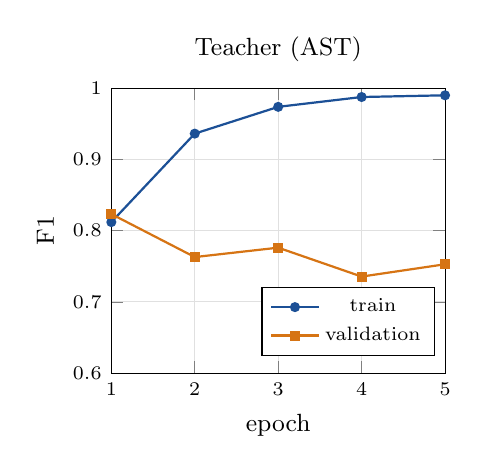
\begin{tikzpicture}
\begin{axis}[
  width=0.48\textwidth, height=5.2cm,
  title={\small Teacher (AST)},
  xlabel={epoch}, ylabel={F1},
  xmin=1, xmax=5, ymin=0.6, ymax=1.0,
  legend style={font=\scriptsize, at={(0.97,0.06)}, anchor=south east},
  grid=major, grid style={black!12},
  tick label style={font=\scriptsize}, label style={font=\small},
]
\addplot[kpblue, thick, mark=*, mark size=1.4pt] coordinates
  {(1,0.8120)(2,0.9362)(3,0.9738)(4,0.9876)(5,0.9900)};
\addlegendentry{train}
\addplot[kporange, thick, mark=square*, mark size=1.4pt] coordinates
  {(1,0.8233)(2,0.7629)(3,0.7761)(4,0.7355)(5,0.7528)};
\addlegendentry{validation}
\end{axis}
\end{tikzpicture}
\hfill
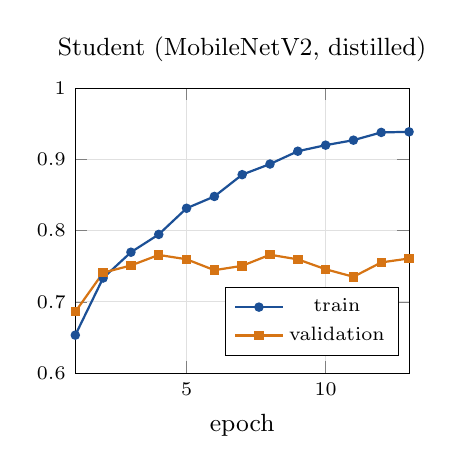
\begin{tikzpicture}
\begin{axis}[
  width=0.48\textwidth, height=5.2cm,
  title={\small Student (MobileNetV2, distilled)},
  xlabel={epoch},
  xmin=1, xmax=13, ymin=0.6, ymax=1.0,
  legend style={font=\scriptsize, at={(0.97,0.06)}, anchor=south east},
  grid=major, grid style={black!12},
  tick label style={font=\scriptsize}, label style={font=\small},
]
\addplot[kpblue, thick, mark=*, mark size=1.3pt] coordinates
  {(1,0.6533)(2,0.7335)(3,0.7697)(4,0.7947)(5,0.8314)(6,0.8480)(7,0.8786)
   (8,0.8935)(9,0.9115)(10,0.9200)(11,0.9270)(12,0.9379)(13,0.9387)};
\addlegendentry{train}
\addplot[kporange, thick, mark=square*, mark size=1.3pt] coordinates
  {(1,0.6861)(2,0.7410)(3,0.7511)(4,0.7659)(5,0.7598)(6,0.7445)(7,0.7506)
   (8,0.7662)(9,0.7597)(10,0.7458)(11,0.7352)(12,0.7554)(13,0.7609)};
\addlegendentry{validation}
\end{axis}
\end{tikzpicture}
\caption{Training dynamics (F1 per epoch, from \texttt{training\_log.csv}).
Left: the teacher peaks at epoch 1 and overfits immediately --- it is
data-limited. Right: the distilled student improves steadily to its best epoch
(8) with a stable validation plateau.}
\label{fig:curves}
\end{figure}

\subsection{Decision-threshold governance}\label{sec:threshold}

The operating threshold was swept \textbf{on the validation set only}; the
test set was never consulted. The sweep (Figure~\ref{fig:sweep}) selects
$\tau^\ast = 0.44$ (val F1 $0.7747$), lifting test F1 from $0.7226$ (at the
0.50 default) to $\mathbf{0.7318}$. A documented low-false-alarm alternative
exists at $\tau = 0.87$ (val FPR $0.098$) but collapses recall to $0.493$ and
is rejected for the primary use case.

\begin{figure}[t]
\centering
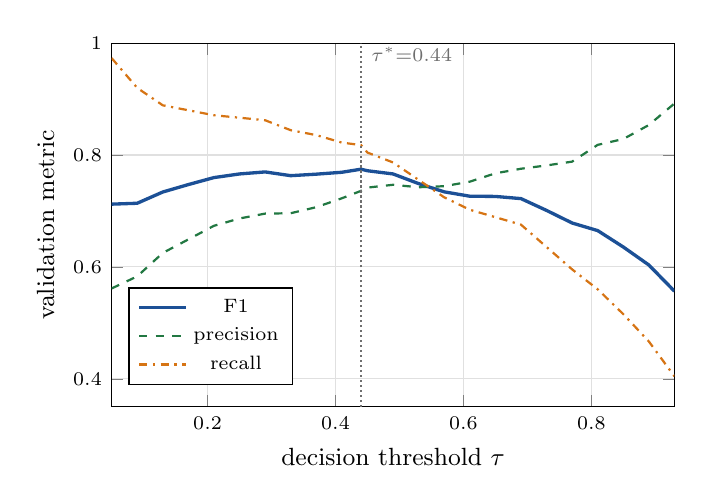
\begin{tikzpicture}
\begin{axis}[
  width=0.72\textwidth, height=6.2cm,
  xlabel={decision threshold $\tau$}, ylabel={validation metric},
  xmin=0.05, xmax=0.93, ymin=0.35, ymax=1.0,
  legend style={font=\scriptsize, at={(0.03,0.06)}, anchor=south west},
  grid=major, grid style={black!12},
  tick label style={font=\scriptsize}, label style={font=\small},
]
\addplot[kpblue, very thick] coordinates
  {(0.05,0.7122)(0.09,0.7138)(0.13,0.7339)(0.17,0.7472)(0.21,0.7597)
   (0.25,0.7662)(0.29,0.7698)(0.33,0.7631)(0.37,0.7658)(0.41,0.7692)
   (0.44,0.7747)(0.45,0.7719)(0.49,0.7662)(0.53,0.7489)(0.57,0.7342)
   (0.61,0.7264)(0.65,0.7260)(0.69,0.7221)(0.73,0.7010)(0.77,0.6785)
   (0.81,0.6649)(0.85,0.6356)(0.89,0.6034)(0.93,0.5566)};
\addlegendentry{F1}
\addplot[kpgreen, thick, dashed] coordinates
  {(0.05,0.5615)(0.09,0.5831)(0.13,0.6250)(0.17,0.6492)(0.21,0.6735)
   (0.25,0.6866)(0.29,0.6953)(0.33,0.6960)(0.37,0.7068)(0.41,0.7227)
   (0.44,0.7360)(0.45,0.7418)(0.49,0.7468)(0.53,0.7424)(0.57,0.7443)
   (0.61,0.7524)(0.65,0.7673)(0.69,0.7755)(0.73,0.7814)(0.77,0.7882)
   (0.81,0.8182)(0.85,0.8286)(0.89,0.8537)(0.93,0.8922)};
\addlegendentry{precision}
\addplot[kporange, thick, dash dot] coordinates
  {(0.05,0.9733)(0.09,0.9200)(0.13,0.8889)(0.17,0.8800)(0.21,0.8711)
   (0.25,0.8667)(0.29,0.8622)(0.33,0.8444)(0.37,0.8356)(0.41,0.8222)
   (0.44,0.8178)(0.45,0.8044)(0.49,0.7867)(0.53,0.7556)(0.57,0.7244)
   (0.61,0.7022)(0.65,0.6889)(0.69,0.6756)(0.73,0.6356)(0.77,0.5956)
   (0.81,0.5600)(0.85,0.5156)(0.89,0.4667)(0.93,0.4044)};
\addlegendentry{recall}
\draw[kpgray, thick, densely dotted]
  (axis cs:0.44,0.35) -- (axis cs:0.44,1.0)
  node[pos=0.97, right, font=\scriptsize, text=kpgray] {$\tau^\ast{=}0.44$};
\end{axis}
\end{tikzpicture}
\caption{Validation threshold sweep for the FP32 student
(\texttt{student\_threshold\_sweep.csv}, downsampled for legibility).}
\label{fig:sweep}
\end{figure}

\subsection{INT8 static post-training quantization}\label{sec:quant}

An initial attempt with \emph{dynamic} PTQ broke the model outright: dynamic
mode quantizes weights only and leaves activation ranges to be computed on the
fly, which is inappropriate for convolutional feature maps whose ranges must
be fixed and calibrated. The shipped artifact instead uses \textbf{static
PTQ}: observers inserted, \textbf{500 real training clips} run through the
network for calibration, weights and activations converted to INT8, and the
result exported as TorchScript (2.80\,MB).

Two engine-level facts dominate deployment (Section~\ref{sec:packaging}): the
artifact was packed with the \texttt{fbgemm} (x86) engine, and under ARM's
\texttt{qnnpack} engine it loads but emits collapsed, meaningless
probabilities ($\sim$0.01 for all inputs; verified empirically). The INT8
output grid is also coarse near the decision boundary
($\approx 0.216$ per logit step, i.e.\ $\approx$5 percentage points of
probability), which interacts with the threshold discussion in
Section~\ref{sec:limits}.

% -----------------------------------------------------------------------------
\section{Results}\label{sec:results}

\subsection{Headline metrics}

\begin{table}[h]
\centering\small
\setlength{\tabcolsep}{4.5pt}
\begin{tabular}{@{}lllrrrrrr@{}}
\toprule
\textbf{Model} & $\tau$ & \textbf{Size} & \textbf{F1} & \textbf{Acc} &
\textbf{Prec} & \textbf{Rec} & \textbf{AUC} & \textbf{ms/clip} \\
\midrule
AST teacher (86.2\,M)        & 0.50 & $\sim$329\,MiB & \textbf{0.8129} & 0.8200 & 0.8462 & 0.7822 & 0.8976 & --- \\
Student FP32 (2.23\,M)       & 0.50 & 8.49\,MB       & 0.7226 & 0.7356 & 0.7598 & 0.6889 & 0.8018 & 57.3 \\
Student FP32, tuned          & 0.44 & 8.49\,MB       & \textbf{0.7318} & 0.7378 & 0.7488 & 0.7156 & 0.8018 & 57.3 \\
Student INT8 (static PTQ)    & 0.50 & \textbf{2.80\,MB} & 0.6910 & 0.7178 & 0.7634 & 0.6311 & --- & \textbf{25.5} \\
\bottomrule
\end{tabular}
\caption{Test-set results (450 balanced clips). Latency is single-thread x86
CPU, measured over the full test pass
(\texttt{quantization\_report.json}).}
\label{tab:results}
\end{table}

Distillation retains $89.0\%$ of the teacher's F1 in $2.6\%$ of its
parameters; quantization then trades a further $0.032$ F1 for a $67.0\%$ size
cut and a $2.25\times$ latency win. The INT8 artifact preserves
\emph{precision} ($0.763$, the best of all student rows) while giving up
recall --- consistent with quantization eroding low-confidence positive
probabilities near the boundary rather than corrupting confident detections.

\subsection{Confusion structure}

\begin{figure}[h]
\centering
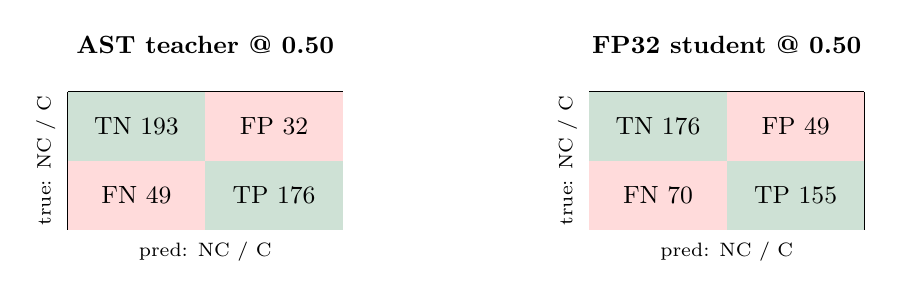
\begin{tikzpicture}[scale=0.92]
\small
% teacher matrix
\begin{scope}
\node[font=\small\bfseries] at (1.9,2.55) {AST teacher @ 0.50};
\draw (0,0) grid[step=1.9] (3.8,1.9);
\fill[kpgreen!22] (0,0.95) rectangle (1.9,1.9);   \node at (0.95,1.425) {TN 193};
\fill[red!14]     (1.9,0.95) rectangle (3.8,1.9); \node at (2.85,1.425) {FP 32};
\fill[red!14]     (0,0) rectangle (1.9,0.95);     \node at (0.95,0.475) {FN 49};
\fill[kpgreen!22] (1.9,0) rectangle (3.8,0.95);   \node at (2.85,0.475) {TP 176};
\node[rotate=90, font=\scriptsize] at (-0.3,0.95) {true: NC / C};
\node[font=\scriptsize] at (1.9,-0.3) {pred: NC / C};
\end{scope}
% student matrix
\begin{scope}[xshift=7.2cm]
\node[font=\small\bfseries] at (1.9,2.55) {FP32 student @ 0.50};
\draw (0,0) grid[step=1.9] (3.8,1.9);
\fill[kpgreen!22] (0,0.95) rectangle (1.9,1.9);   \node at (0.95,1.425) {TN 176};
\fill[red!14]     (1.9,0.95) rectangle (3.8,1.9); \node at (2.85,1.425) {FP 49};
\fill[red!14]     (0,0) rectangle (1.9,0.95);     \node at (0.95,0.475) {FN 70};
\fill[kpgreen!22] (1.9,0) rectangle (3.8,0.95);   \node at (2.85,0.475) {TP 155};
\node[rotate=90, font=\scriptsize] at (-0.3,0.95) {true: NC / C};
\node[font=\scriptsize] at (1.9,-0.3) {pred: NC / C};
\end{scope}
\end{tikzpicture}
\caption{Test confusion matrices (NC = \notcooking{}, C = \cooking{};
225 clips per class). Both models err more by \emph{missing} cooking than by
false alarms.}
\label{fig:confusion}
\end{figure}

\subsection{Where the errors live}\label{sec:errors}

Errors concentrate almost entirely in the by-design hard regime: on type-C
clips (cooking overlapped with a competing sound at SNR down to $-5$\,dB;
17\% of the corpus) accuracy drops to roughly \textbf{39--50\%}, versus
\textbf{75--78\%} on clean, non-overlapping clips. Two structural factors
compound this: the \notcooking{} class is an unstructured 1{,}160-sound pool
(harder to characterize than the 10 curated cooking subtypes), and the
teacher itself is data-limited (Section~\ref{sec:teacher}), capping the soft
targets the student can learn from.

% -----------------------------------------------------------------------------
\section{Deployment}\label{sec:deploy}

\subsection{One \texttt{Predictor}, everywhere}\label{sec:parity}

All consumers --- \texttt{inference/predict.py}, batch evaluation, and the
Telegram bot --- import the same \texttt{kitpri.inference.Predictor}, which
owns audio decoding, resampling, the mel pipeline of
Table~\ref{tab:preproc}, model loading, and thresholding. Preprocessing drift
between training and serving is therefore structurally impossible rather than
procedurally discouraged. Parity was verified empirically: 6/6 exact
prediction matches against the archived training-time evaluation and a
maximum absolute probability difference of $0.00148$ over a 20-clip audit.

\subsection{Packaging and the x86 guard}\label{sec:packaging}

\begin{itemize}[itemsep=2pt,topsep=3pt]
  \item \textbf{Docker}: a \texttt{python:3.11-slim} image pinned to
        \texttt{--platform linux/amd64}, installing CPU-only torch wheels;
        \texttt{libsndfile1} and \texttt{ffmpeg} are the only system
        dependencies.
  \item \textbf{ARM refusal}: because the INT8 artifact is
        \texttt{fbgemm}-packed (Section~\ref{sec:quant}),
        \texttt{predict.py} detects non-x86 hosts and \emph{refuses} to run
        INT8 there --- failing loudly instead of returning collapsed
        probabilities --- and directs the user to \texttt{--model fp32} or
        the Docker container. The FP32 student runs correctly on any
        architecture.
  \item \textbf{SmartThings path}: the production target is ARM, so the
        deployable INT8 artifact must be re-quantized with
        \texttt{qnnpack} (config already provisioned:
        \texttt{configs/experiments/quantize.yaml} sets
        \texttt{backend: qnnpack}); this is scheduled future work.
\end{itemize}

\subsection{Live demonstration: Telegram bot}\label{sec:bot}

The public bot (\texttt{@kitpribot}) accepts voice messages and audio files
(\texttt{.wav}/\texttt{.mp3}/\texttt{.ogg}/\texttt{.m4a}/\texttt{.flac}),
runs the FP32 student at $\tau=0.44$ through the shared \texttt{Predictor},
and replies \cooking{}/\notcooking{}. It uses \texttt{python-telegram-bot}
v22 with \emph{long polling}: the process makes outbound HTTPS calls to the
Telegram API and requires \textbf{no public URL, webhook, TLS certificate, or
open inbound port} --- a property that makes the hosting architecture below
essentially configuration-free.

Operational hygiene worth recording: the bot token is provided exclusively
via environment variable (never argv, which is visible in \texttt{ps});
\texttt{httpx} request logging is silenced because Telegram API URLs embed
the token; and exactly \emph{one} poller may consume a token at a time ---
Telegram rejects concurrent \texttt{getUpdates} consumers with HTTP 409.

\subsection{Always-on cloud hosting at \$0}\label{sec:cloud}

The bot initially ran on a developer laptop, making demo availability
hostage to that laptop's lid. It now runs 24/7 on an \textbf{Oracle Cloud
Infrastructure Always-Free} VM (Table~\ref{tab:vm}), surviving crashes,
reboots, and developer absence, at zero recurring cost.

\begin{table}[h]
\centering\small
\begin{tabular}{@{}ll@{}}
\toprule
Shape / region   & VM.Standard.E2.1.Micro (1 OCPU x86, 954\,MB RAM), ap-hyderabad-1 \\
OS / runtime     & Ubuntu 24.04 LTS · Python 3.12 venv · \texttt{torch} 2.13 (CPU wheels) \\
Memory strategy  & 2\,GB swapfile provisioned before dependency install (1\,GB RAM alone \\
                 & is insufficient for torch import + model load headroom) \\
Supervision      & systemd unit \texttt{kitpri-bot.service}: \texttt{Restart=always}, \\
                 & \texttt{RestartSec=5}, enabled at boot, journald logging \\
Shutdown quirk   & \texttt{TimeoutStopSec=15}: PTB's graceful shutdown can hang on \\
                 & SIGTERM; systemd escalates to SIGKILL, preventing zombie pollers \\
Secrets          & token in \texttt{.env} (mode 600), delivered by \texttt{scp}, injected via \\
                 & systemd \texttt{EnvironmentFile}; never in the repository or logs \\
Network exposure & \textbf{none inbound} --- long polling is outbound-only \\
Steady-state RAM & $\approx$674\,MB used including OS; model load $\approx$7\,s on 1 core \\
Cost             & \$0 (Always Free tier, no time limit) \\
\bottomrule
\end{tabular}
\caption{Production hosting of the demonstration bot.}
\label{tab:vm}
\end{table}

\begin{figure}[h]
\centering
\begin{tikzpicture}[
  node distance=6mm and 12mm,
  box/.style={draw, rounded corners=2pt, align=center, font=\small,
              minimum height=9mm, inner sep=5pt},
  arr/.style={{Stealth[length=2.4mm]}-{Stealth[length=2.4mm]}, thick, kpgray}
]
\node[box, fill=kpblue!12] (user) {User's phone\\ \footnotesize voice note / audio file};
\node[box, fill=kpgray!14, right=of user] (tg) {Telegram\\ Bot API};
\node[box, fill=kpgreen!14, right=of tg, text width=4.6cm]
  (vm) {Oracle Always-Free VM\\[1pt]
        \footnotesize systemd $\rightarrow$ \texttt{bot.py} $\rightarrow$ \texttt{Predictor}\\
        \footnotesize FP32 student · $\tau{=}0.44$ · CPU};
\draw[arr] (user) -- (tg);
\draw[arr] (tg) -- node[above, font=\scriptsize, text=kpgray]
  {outbound long poll} (vm);
\node[below=2.5mm of vm, font=\scriptsize, text=kpgray]
  {no inbound ports · no webhook · no public URL};
\end{tikzpicture}
\caption{Serving topology. The VM initiates all connections; the demo
survives laptop shutdown, process crashes (systemd restart), and VM reboots
(service enabled at boot).}
\label{fig:hosting}
\end{figure}

The deployment is reproducible from two committed artifacts: a step-by-step
guide (\texttt{telegram\_bot/DEPLOY.md}) and the systemd unit
(\texttt{telegram\_bot/kitpri-bot.service}); local development retains the
\texttt{start.sh} launcher, with the operational rule that the laptop poller
must be stopped whenever the cloud poller is active (the 409-conflict
constraint of Section~\ref{sec:bot}).

% -----------------------------------------------------------------------------
\section{Limitations and Future Work}\label{sec:limits}

Reported openly rather than omitted:

\begin{enumerate}[itemsep=3pt,topsep=3pt]
  \item \textbf{Overlapped audio dominates the error budget.} Type-C clips
        (17\% of data, SNR down to $-5$\,dB) score 39--50\% accuracy versus
        75--78\% on clean clips. This difficulty is intentional --- it is the
        deployment reality the model must eventually master --- but it is not
        yet mastered.
  \item \textbf{Unstructured negatives.} The \notcooking{} pool is a single
        heterogeneous 1{,}160-clip set; curating it into subtypes (as was done
        for \cooking{}) would likely sharpen the boundary.
  \item \textbf{The teacher is data-limited.} Val F1 peaks at epoch 1
        (Figure~\ref{fig:curves}); more diverse data and stronger
        augmentation --- not a larger model --- are the indicated remedies.
  \item \textbf{INT8 threshold not independently re-tuned.} $\tau^\ast=0.44$
        was selected on FP32 validation probabilities. Quantization shifts
        calibration and coarsens the probability grid
        ($\approx$5 points near the boundary), so an INT8-specific sweep is
        outstanding.
  \item \textbf{Recall below production bar.} The FP32 student misses
        $\approx$28\% of cooking events at $\tau=0.44$; INT8 misses
        $\approx$37\% at 0.50. This milestone demonstrates a working
        end-to-end pipeline, not a shippable detector.
  \item \textbf{INT8 artifact is x86-only.} \texttt{fbgemm}-packed; the ARM
        (SmartThings) target requires \texttt{qnnpack} re-quantization or
        quantization-aware training. The refusal guard prevents silent
        failure meanwhile.
  \item \textbf{Licensing.} Negatives derive from ESC-50 (CC BY-NC 3.0);
        commercial deployment requires re-sourcing negative audio.
\end{enumerate}

\noindent\textbf{Future work}, in priority order: \texttt{qnnpack}
re-quantization for the ARM target; INT8-specific threshold re-sweep;
recall-focused data expansion (more type-C-like training signal, curated
negative subtypes); quantization-aware training if PTQ remains the
bottleneck.

% -----------------------------------------------------------------------------
\section{Conclusion}\label{sec:conclusion}

KitPri v4 demonstrates the full arc from research-grade transformer to
edge-deployable artifact: a 329\,MiB AST teacher distilled and quantized into
a 2.80\,MB TorchScript model --- $>118\times$ smaller, $2.25\times$ faster ---
while retaining $85\%$ of the teacher's test F1 (INT8 at the default
threshold) and $90\%$ in FP32 form with governed threshold tuning. Equal
engineering weight was placed on what surrounds the model: a deliberately
hard synthetic-mixture dataset, one shared preprocessing/serving code path
with verified parity, loud failure on unsupported hardware, and a
zero-cost, always-on public demonstration under systemd supervision on
Oracle's free tier. The limitations register makes the remaining distance to
production explicit --- ARM re-quantization, recall recovery, and negative-class
curation --- and each item is scoped against a config or script already
provisioned in the repository.

% -----------------------------------------------------------------------------
\begin{thebibliography}{9}\small

\bibitem{gong2021ast}
Y.~Gong, Y.-A.~Chung, and J.~Glass,
``AST: Audio Spectrogram Transformer,''
\emph{Proc. Interspeech}, 2021.

\bibitem{sandler2018mobilenetv2}
M.~Sandler, A.~Howard, M.~Zhu, A.~Zhmoginov, and L.-C.~Chen,
``MobileNetV2: Inverted Residuals and Linear Bottlenecks,''
\emph{Proc. CVPR}, 2018.

\bibitem{hinton2015distilling}
G.~Hinton, O.~Vinyals, and J.~Dean,
``Distilling the Knowledge in a Neural Network,''
\emph{NIPS Deep Learning Workshop}, 2015. arXiv:1503.02531.

\bibitem{piczak2015esc}
K.~J.~Piczak,
``ESC: Dataset for Environmental Sound Classification,''
\emph{Proc. ACM Multimedia}, 2015. Licensed CC BY-NC 3.0.

\bibitem{pytorch-quant}
PyTorch Team,
``Quantization --- PyTorch documentation,''
\url{https://pytorch.org/docs/stable/quantization.html}.

\bibitem{timm}
R.~Wightman,
``PyTorch Image Models (timm),''
\url{https://github.com/huggingface/pytorch-image-models}.

\end{thebibliography}

\end{document}
